%User manuals for the different clients. Directed towards users (includes everyone). Start with subsection here.

%This chapter explains to the user how each client should be used. It starts with the desktop and web clients. These clients are the main clients that can handle the main features. Then comes instructions for the mobile clients that are designed to search for files and tell the server to convert them.

This chapter explains how you use each of the \appName\ clients. First instructions on how to use the desktop and the web clients are presented. These are the clients which provide the most functionality. The mobile clients are more lightweight and offer a subset of the functionality presented by the desktop client. Instructions on using the smartphone applications for \term{Android} and \term{iOS} are presented in their on sections at the end of the chapter. 


\section{Desktop}
This is a user manual for the desktop client. It will provide guides on how to use the client and the different functionalities it holds. The screenshots shown in this document are made from a Linux machine, but the Desktop application also runs on Windows or Mac, and will follow the design priciples thereafter. Because of this, the look of the client may vary, but the functionality is the same, and hopefully this manual will be of service anyways. 

\subsection{Login and startup}
When you start this application the first thing that's displayed is a login screen, as illustrated in \refer{fig:des_login-pic}. In this screen you enter your username, password and the IP-Address for the server and then press login to enter the Genomizer Desktop.

\begin{figure}[htb]
	\addScaledImage{0.5}{des_loginpicture.png}
	\caption{Screenshot of the login screen.}
	\label{fig:des_login-pic}
\end{figure}
The application is built with tabs, as illustrated below in the upper part of \refer{fig:des_desktop-view}. Each tab contains separate features of the application. There are six tabs: Search, Upload, Process, Workspace, Analyze and Administration.
\begin{figure}[htb]
	\addImage{des_searchtab.png}
	\caption{Illustration of the different tabs of Genomizer Desktop and displaying the Search tab.}
	\label{fig:des_desktop-view}
\end{figure}
\FloatBarrier

\subsection{Search}
The first tab that meets the user after logging in is the Search tab, illustrated in \refer{fig:des_desktop-view}. The Search tab uses the same query building technique as the “Pubmed Advanced Search Builder”. It has one text field where you either can type in the query yourself or you can use the query builder below it. Each row in the query builder has at most five components. These are a logical expression, an annotation name field, a free text field or a drop down menu to insert search words, a minus button and a plus button. The minus button removes a row and the plus button adds a row. These buttons are however not available in each row. The plus button is only available in the last row. The minus button is available in every row except if there is only one row in the query builder. The logical expressions combines the annotations, so they are available in every row but the first.
By writing in the annotation text field or selecting a value in the drop down menu you can specify the query the row will produce. Together each row builds a full query. As illustrated in \refer{fig:des_search-query} below.
\begin{figure}[htb]
	\addImage{des_searchtab.png}
	\caption{Illustration of a query, made by the query builder.}
	\label{fig:des_search-query}
\end{figure}
\FloatBarrier

\subsection{Upload}
If the user needs to upload a file to the database it can be done through the upload tab.
When the tab is pressed the user gets presented with a text field and a button where they can search for an existing experiment to upload to and another button for adding a new experiment. When the user presses the new experiment button, the user is presented with annotations they can choose between. If they pressed the existing experiment button, they are instead presented with annotations they can't choose between. They are also presented with buttons named Select files and Upload selected files, with which the user can choose a file via a file browser and upload them. The upload tab is illustrated in \refer{fig:des_upload-view} and the file browser is illustrated in \refer{fig:des_upload}.
\begin{figure}[htb]
	\addImage{des_uploadexisting.png}
	\caption{Illustration of the upload tab where the browse and upload functions are shown.}
	\label{fig:des_upload-view}
\end{figure}

\begin{figure}[htb]
	\addScaledImage{0.4}{des_uploadselect.png}
	\caption{Choosing a file for uploading}
	\label{fig:des_upload}
\end{figure}
\FloatBarrier

\subsection{Process}
In the process tab there is a list called Files that on the left side of the tab. From this list the user can mark RAW-files and choose to create profile data. By left clicking on the files they will be marked. If the user left clicks once again on the same file it will be unmarked. If the user then presses the Create profile data button which is visable in the middle of the tab see \refer{fig:des_process-view}, all the files that are marked will now be processed to profile data. This list of files will be empty unless the user has chosen to process selected RAW-files from the workspace tab. If that is the case then those selected RAW-files will then be visable in the list of files in the process tab. When the user has selected some RAW files the user has the option to change conversion parameters that is above the create profile data button as illustrated in \refer{fig:des_process-view}. These parameters has pre-set values. The conversion parameters are Flags, Genome release files, Window size,Smooth type,Step position,Step size,Print mean and Print zeros. If the user has selected some RAW-files and pressed the Create profile button, then if all went well and the server could convert the files a message "The server has converted: filename" will print in Convert Files for each file that was converted to profile data. If for some reason the server couldn't create profile data for any RAW-file another message "WARNING - The server couldn't convert: filename" will print in Convert Files that is visible in the middle bottom of the process tab see \refer{fig:des_process-view}.


\begin{figure}[htb]
	\addImage{des_processtab.png}
	\caption{Screenshot of the process tab in the program.}
	\label{fig:des_process-view}
\end{figure}
\FloatBarrier

\subsection{Workspace}
The Workspace View is the heart of the application for the user. Chosen files from the search is collected in this view, and the user can choose different options to process and analyze the data. 
For now, the only function here that is implemented is Download, but more will come.
\subsubsection{Download}
The user can make the choice to download. If the user presses the DOWNLOAD SELECTED button seen in \refer{fig:des_workspace-view}, then a pop up menu will present it self to the user as illustrated in \refer{fig:des_download-view}. In the pop up menu, the files that were selected in the workspace will be shown, then the user can choose a file format for each of the files (this functionality is not yet implemented). If the download button is pressed, the user gets to choose a directory where the files will be saved. When a directory has been chosen, the files get downloaded and saved in folders named after the experiments in which they belong. 
\begin{figure}[htb]
	\addImage{des_workspaceselect.png}
	\caption{Screenshot of the workspace tab in the program.}
	\label{fig:des_workspace-view}
\end{figure}
\begin{figure}[htb]
	\addImage{des_download.png}
	\caption{The download files pop up menu}
	\label{fig:des_download-view}
\end{figure}
\FloatBarrier

\subsection{Administration}
The system administration tools for the desktop client is available under the Administration tab. When a user selects the add button in the sidepanel a new popup windows appears. It is possible to write the name of the new annotation and name of new categories in this popup, as well as check a forced annotation box. See \refer{fig:adm_desktopgui}.
\begin{figure}[h!]
\addImage{des_addAnnotation.png}
\caption{The add new annotation popup.}
\label{fig:adm_desktopgui}
\end{figure}

\FloatBarrier

\section{Web}
To access the web application, navigate to a domain and directory that publicly serves the web page. An example of this is the “official” test enviroment: www8.cs.umu.se/~oi11lsm/app/.
All functionality of the web application is (or rather should be) fairly self-explanatory and intuitive. A short description and explanation will be given for each component that have been implemented so far.
\subsection{Using the interface}
This section will describe how to use the interface and how to interact with it.
\subsubsection{Start view}
%figure 2
\begin{figure}[h]
\centering
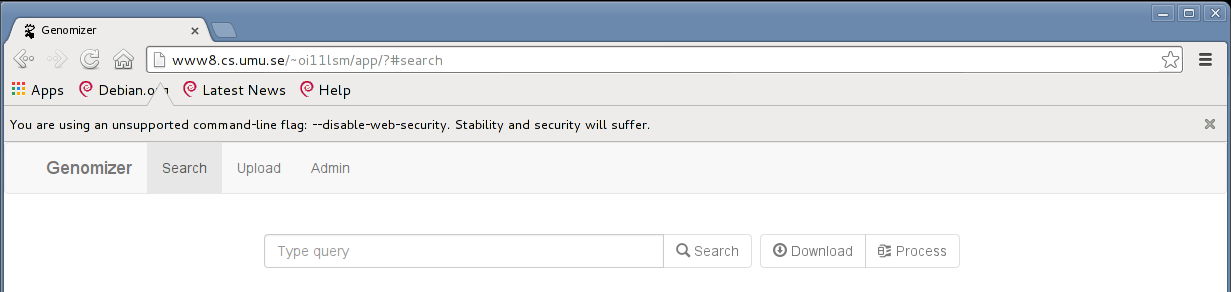
\includegraphics[width=1\textwidth]{web_search_welcome.png}
\caption{\label{fig:web_search_welcome} The welcome screen of the webpage.}
\end{figure}

When the website has loaded, the user is taken to the search page as shown in \refer{fig:web_search_welcome}.

The navigation bar at the top has three buttons with the following functionality:
\begin{itemize}
	\item Clicking the “Genomizer” logo should take the user right back to the start view.
	\item The “Search” button will bring up the search view where the user can enter search strings to be sent to the server, and view search results.
	\item The “Upload” button will bring up the upload view where the user can select files to be uploaded and input annotation to a new experiment.
	\item The “Admin” button will be shown for administrators, that is where the administrator can handle users and annotations.
\end{itemize}
This navigation bar is persistent through all subpages and can easily be accessed.

Below the navigation bar a “search-and-functionality” bar is visible, there is a search field and there are three buttons, Search, Download and process. However, when first entering the page the buttons will be disabled. When you enter something in the search field the search button will become enabled and clickable. 
When the user wants to search for something he can simply write a search query in pubmed style(ex; Exp1[ExpID]) in the search field and either press enter or click the Search button. 

%figure BILD
\begin{figure}[h]
\centering
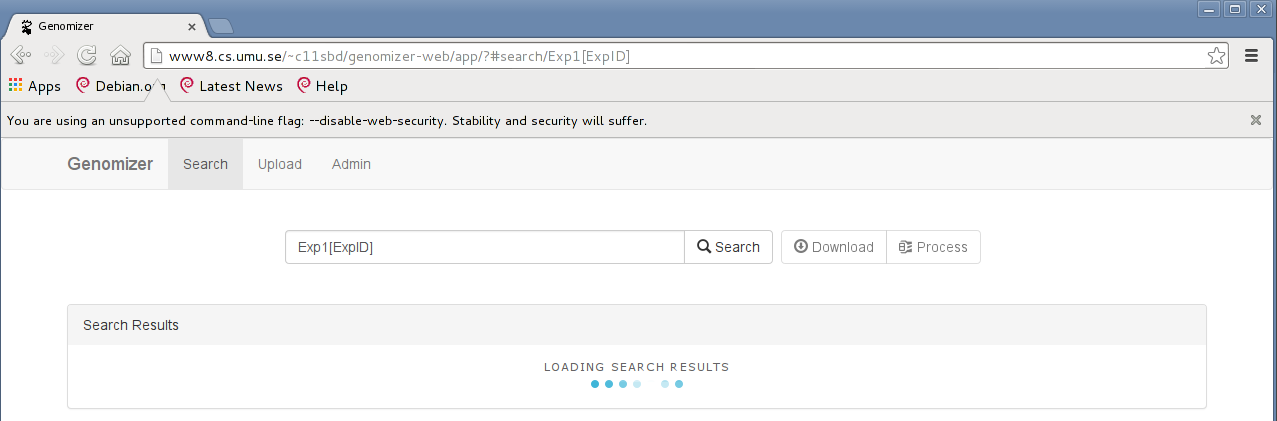
\includegraphics[width=1\textwidth]{web_search_searching.png}
\caption{\label{fig:web_search_searching}will be shown while searching for data in the database before any results are found.}
\end{figure}

After having typed a query and pressed search, the search results will load displaying the loading spinner as can be seen in figure \refer{fig:web_search_searching}.
%figure x3
\begin{figure}[h]
\centering
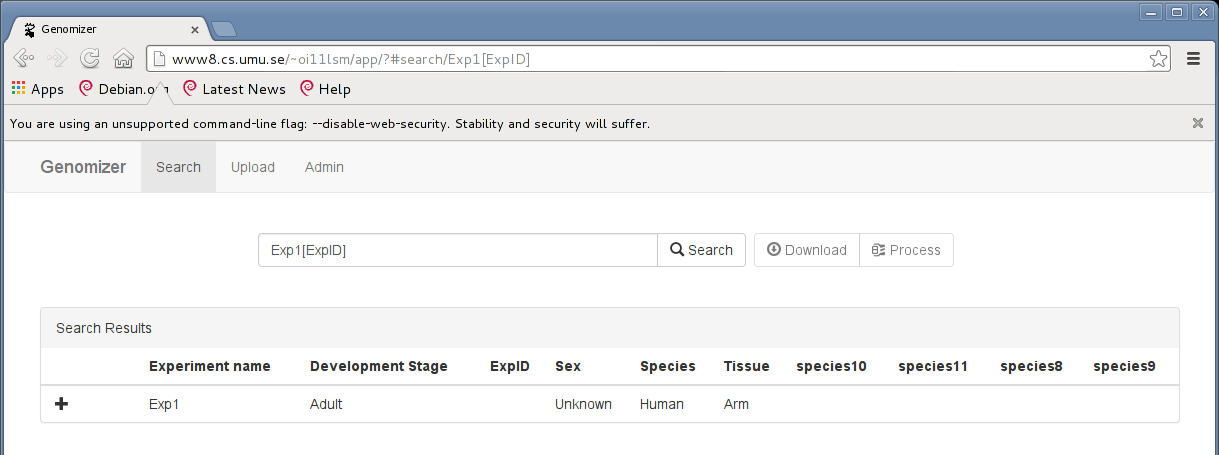
\includegraphics[width=1\textwidth]{web_search_searchTab.png}
\caption{\label{fig:web_search_searchTab}the search tab after a search for ‘Exp1[ExpID]’.}
\end{figure}

The view shown in \refer{fig:web_search_searchTab} contains two major elements; a “search-and-functionality” bar and a list of search results retrieved after searching for ‘Exp1[ExpID]’. The buttons next to the search bar are supposed to do what they say: 
\begin{itemize}
	\item “Search” searches for the query in the search bar. 
	\item “Download” downloads the selected files. 
	\item “Process” brings up a new window in front of the search view with options for file processing. This feature is demonstrated further in Figure \refer{fig:web_process_modal}.
\end{itemize}

Below the search bar in \refer{fig:web_search_searchTab} is the “search results” list. This list contains all experiments returned from a search. Every experiment can be expanded to show the file types it contains,. Each file type can be expanded to show all files of that type in the experiment. Each file has a check box next to it that is used to select files to be processed or downloaded, currently the user is only able to select one file at a time. 
%figure x4
\begin{figure}[h]
\centering
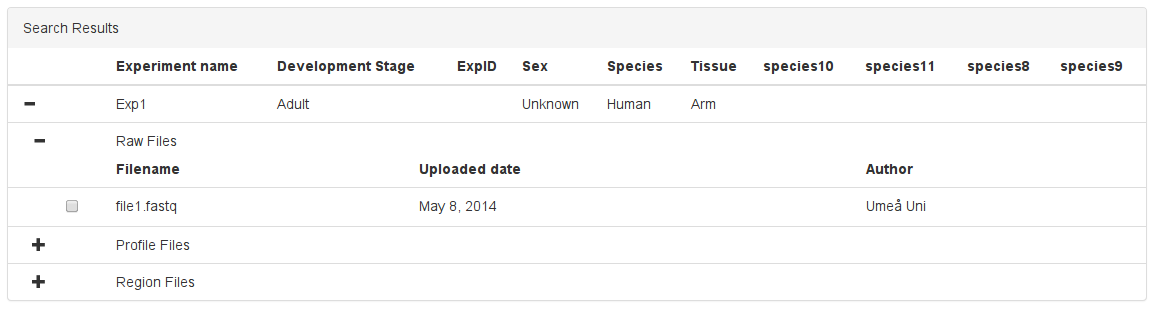
\includegraphics[width=1\textwidth]{web_search_searchResult.png}
\caption{\label{fig:web_search_searchResult}the search results table zoomed in, displaying a raw file’s information after having expanded an experiment.}
\end{figure}

If a search is successful, you will be met with a table of results. This table has a header displaying the annotation types. Below that, all the experiments returned from a search and their corresponding annotation values, as can be seen in \refer{fig:web_search_searchResult}.
%figure BILD PÅ NO SEARCH RESULTS
\begin{figure}[h]
\centering
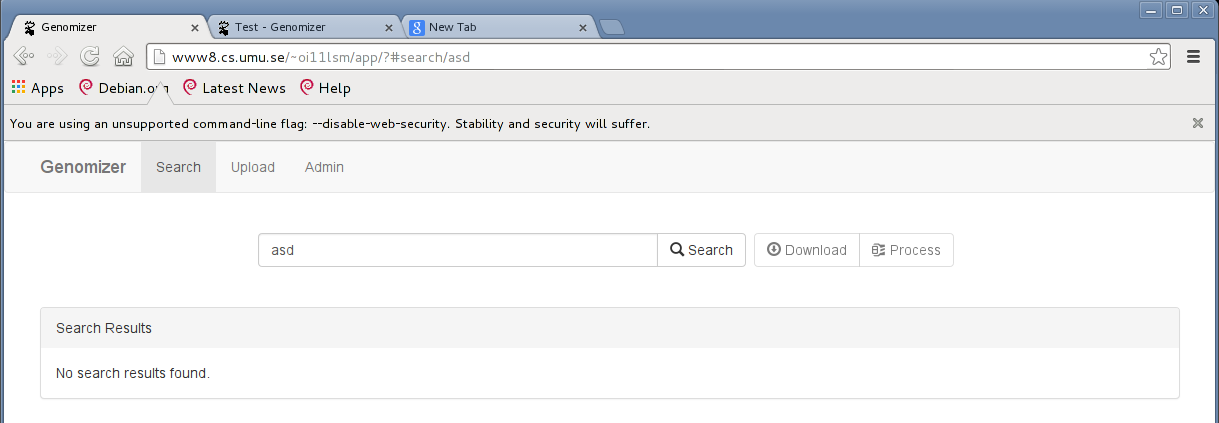
\includegraphics[width=1\textwidth]{web_search_noResult.png}
\caption{\label{fig:web_search_noResult}tells the user that no data was found given the search query entered by the user.}
\end{figure}

If the search is unsuccessful, the Search Results table will be empty stating “No search results found” as can be seen in \refer{fig:web_search_noResult}.

\subsubsection{The processing modal}
%figure X6
\begin{figure}[ht]
\centering
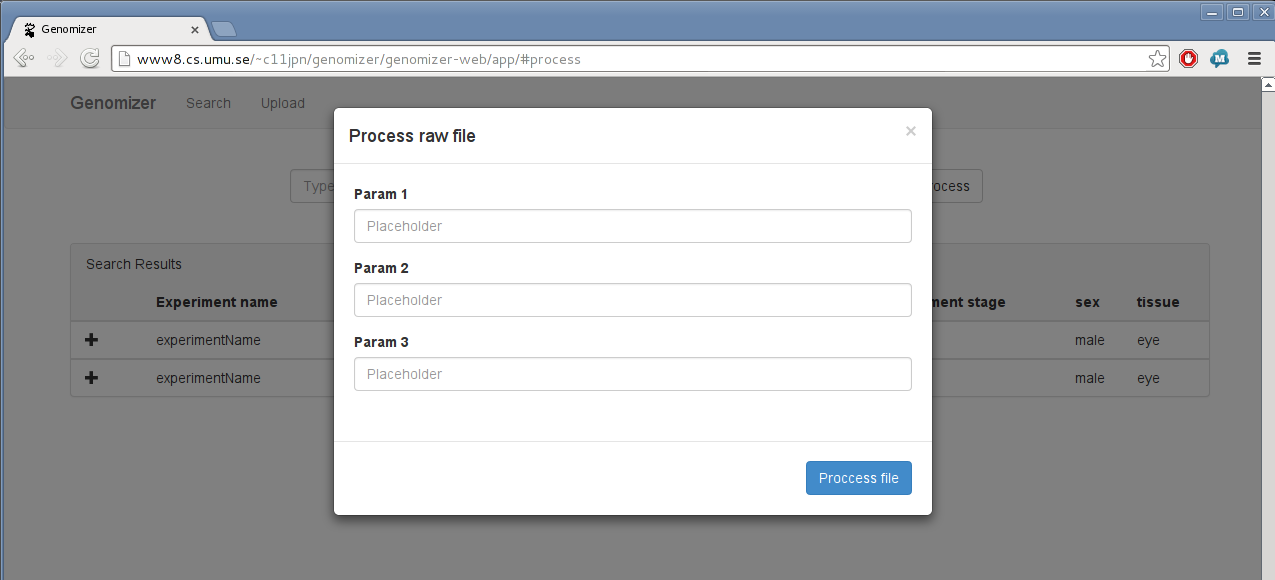
\includegraphics[width=1\textwidth]{web_process_modal.png}
\caption{\label{fig:web_process_modal}The process file modal.}
\end{figure}

The user will be presented with the view in \refer{fig:web_process_modal} when he wants to process one raw file to profile data. The user will already have selected one file he wishes to process and he will enter the parameters for the processing.
\subsubsection{The upload view}
%figure X7
\begin{figure}[h]
\centering
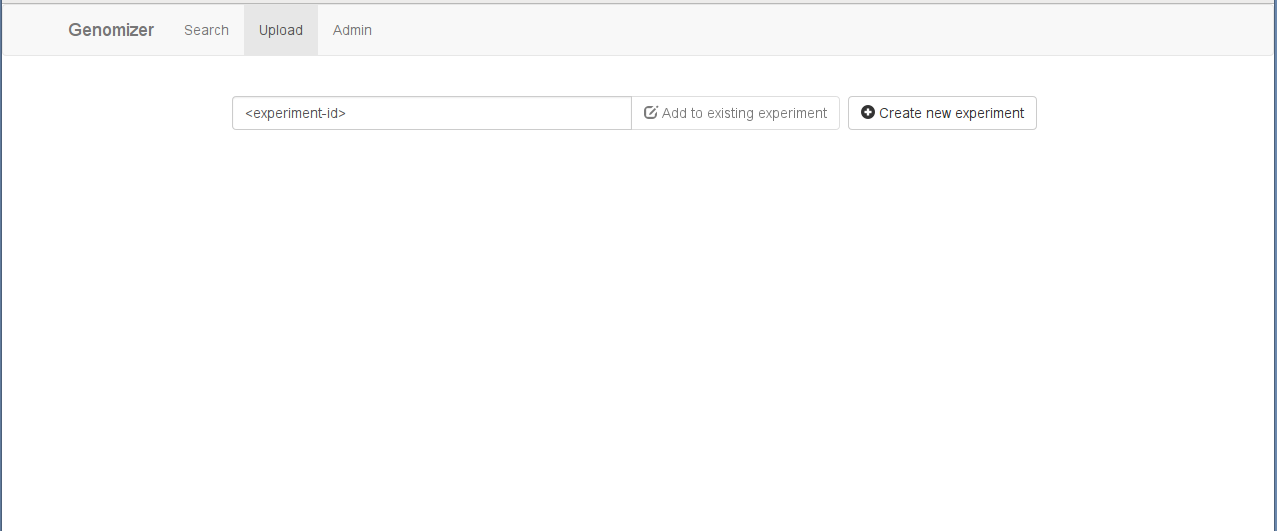
\includegraphics[width=1\textwidth]{web_upload_uploadView.png}
\caption{\label{fig:web_upload_uploadView}The upload view.}
\end{figure}

When the user presses the upload tab in the navigation bar the view in \refer{fig:web_upload_uploadView} will appear. The user has the option to create a new and fresh experiment or to load an existing experiment by entering its experiment ID. 
%figure X8
\begin{figure}[h]
\centering
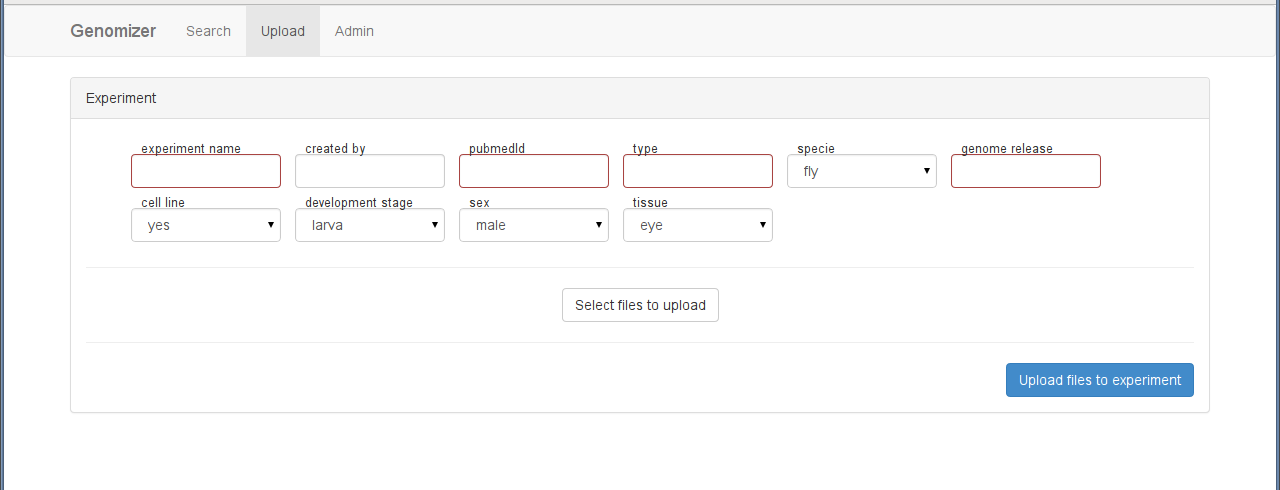
\includegraphics[width=1\textwidth]{web_upload_newExperiment.png}
\caption{\label{fig:web_upload_newExperiment}Creating a new experiment.}
\end{figure}

After clicking the “Create new experiment” button the view in \refer{fig:web_upload_newExperiment} will appear. Here the user can input the annotations for the experiment through either freetext fields or drop-down lists. If a freetext field has a red border around it, that annotation is required and no files can be uploaded before it has been filled in. The user can also browse for local files to upload by clicking the “Select files to upload” button. 
%figure X9
\begin{figure}[h]
\centering
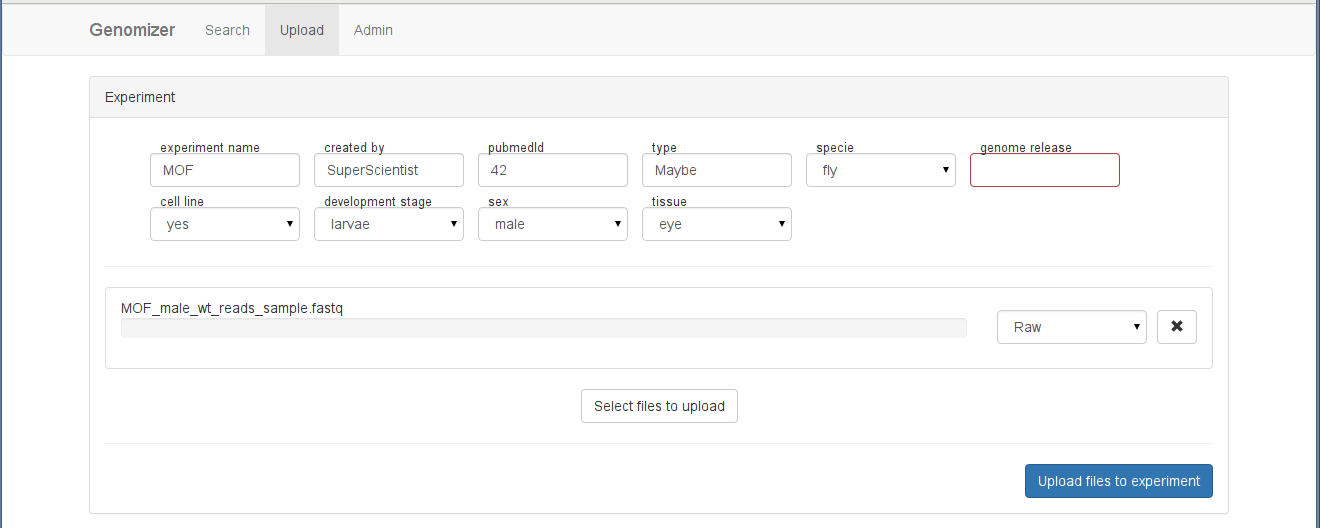
\includegraphics[width=1\textwidth]{web_upload_fileUpload.png}
\caption{\label{fig:web_upload_fileUpload}File selected for upload.}
\end{figure}
 
When the user has selected files, they will appear below the annotations as in Figure \refer{fig:web_upload_fileUpload}. The file’s name is displayed in the top left corner. On the right side there is an option to select what type of file is being uploaded and an option to remove the file from the experiment.

When the user is done selecting files and annotations it can click the “Upload files to experiment” button. The files will then be sent to the server with the specified annotations (this functionality might not be fully working by the time this was written).

\subsubsection{Systemadministration view}

This part of the web application is only accessible if the user have administrator-rights. It is integrated with the rest of the web UI and accessible through an admin-tab. The administrator can through this site see all existing annotations, add new annotations and delete existing ones.
The startpage of this section has a Create new annotations button, a list of existing annotations in the database and an edit button per existing annotation. 
The view currently looks like in figure \refer{adm__web_annotationView}. 

\begin{figure}[h]
 \addImage{web_sysadminAnnotationView.jpg}
 \caption{The startpage for the administrator in the web client}
 \label{adm__web_annotationView}
\end{figure}

For each annotation in the annotations list, an Edit button is available. 
When pressed, it will take you to a page in which you can edit the selected annotation to change its name, 
type and whether it is forced (See \refer{adm_web_editView}). 

\begin{figure}[h]
 \addImage{web_sysadminEditView.jpg}
 \caption{The edit annotation view}
 \label{adm_web_editView}
\end{figure}
\newpage
In the edit page the admin can see the attributes of the chosen annotation and is able to delete the chosen annotation.

If the admin clicks on Create new annotation from the admin startpage, another view will open with the following structure:
\begin{itemize}
 \item Annotation Name
 \subitem Admin can enter a name for the annotation
 
 \item Annotation Types
 \subitem Yes/No/Unknown - this will create a drop-down list with those three options.
 \subitem Freetext - will create an annotation that the users will be able to enter anything.
 \subitem Drop-down list - will enable a fourth field enabling the admin to enter which items that this list will contain.
 
 \item Forced Annotation
 \subitem Admin can choose if the new annotation should be forced for users to enter. 
\end{itemize}

A Create Annotation will, if all necessary information has been entered, result in the annotation to be added to the database. Otherwise the admin will be alerted of the mistake and nothing will be created.
\newpage
A back button which takes the user back to the annotations start page is also available in this view. In figure \refer{adm_web_createView} the create annotation view can be seen.

\begin{figure}[t]
 \addImage{web_sysadminCreateAnnotation.jpg}
 \caption{The view for administrators where new annotations can be created}
 \label{adm_web_createView}
\end{figure}

\subsection{Setting up the application}
To setup the application, move the content of the folder called app in genomizer-web to the desired location from where the application should be run. To run the webpage open a web browser and enter the url to the folder which contains the \texttt{index.html} file(where the content of app was placed).
Ex. given that the genomizer-web folder is placed in my home folder and i want to put the webpage in a folder called public\_html which is also in my home folder. In linux i do the following steps.
\begin{enumerate}
	\item Navigate to the app folder: \texttt{“cd ~/genomizer-web/app/”}
	\item Move the contents of app to the folder called public\_html:\\ \texttt{“mv * ~/public\_html/”}
	\item Given that the url to the pubilc\_html folder is: \\ \filePath{“www8.cs.umu.se/~c11abc/”}
	\item To run the application start a web browser and type \\ \filePath{“www8.cs.umu.se/~c11abc/”}
\end{enumerate}
This will open the webpage in the browser.

\FloatBarrier

\section{Android}
In this section you will find instructions for the usage of the Genomizer android application. \ref{sec:and_start} describes how to start the application and \ref{sec:and_search} gives instructions on how to search for experiments.
\subsection{Start the application}\label{sec:and_start}
Localize the Genomizer icon in the android view of all your installed apps or
use a shortcut on one of your \term{desktop views}. Click the icon in order to start
Genomizer, you will be presented with the login screen.

To start working with your Genomizer app you have to login. If you have a
account with the service: insert your user name and password in the correspond-
ing boxes and press \click{Sign in} to access the application. If you are not yet
registered with the service, ask the system administrator for help with
the creation of your account.
\subsection{Search for files}\label{sec:and_search}
The search view offers a way to find data files with certain attributes. This view is accessed directly after logging in and can be reached at any time by pressing the
search icon on the action bar.

The annotation text fields can be filled in to find files matching the search
criteria. By checking the check box to the right of the annotation field, it gets
activated and appended as part of the search criteria. The functionality can
be used to conduct many similar searches by adding and subtracting criteria as
requested. The search is initiated by pressing \click{Search} at the bottom of the
page.

After pressing Search you will be  redirected to the search results view  that displays a list of available experiments that matches the search annotations. Every experiment is listed showing the experiment name. To receive more information about data files that are available for each experiment, click on an experiment in the list. By clicking an entry you will be taken to a new view displaying all available data files for that experiment. The data files are organised by: raw data, profile data and region data. Every data file got a checkbox next to it.  The checkboxes can be used to select files for conversion. When all files are selected click the \click{Send to conversion} button.

\FloatBarrier

\section{iOS}
In order to use the program import the project from github into Xcode from the following repository:
\url{https://github.com/genomizer/genomizer-iOS.git} 

\begin{figure}[ht]
\addScaledImage{0.2}{ios_login.png}
\caption{The login screen.}
\label{fig:ios_login}
\end{figure}
\FloatBarrier

To compile and run the program press \click{cmd+R}. A simulator will start and the login screen will be shown as seen in \refer{fig:ios_login}  below. A user gets logged in when accepted credentials are entered in the \term{username} and \term{password} fields and the \click{Sign in} button is pressed. If incorrect credentials is entered, a popup message is shown, informing the user that the username or password is incorrect.

\begin{figure}[ht]
\addScaledImage{0.2}{ios_search.png}
\caption{The search screen.}
\label{fig:ios_search}
\end{figure}
\FloatBarrier


After logging in, the user is presented with a search view as seen in \refer{fig:ios_search}. The bottom menu bar is used to navigate between the Search-, Selected files- and More-view according to Apples current GUI standards for iOS 7. In the current state, the More-menu only contains a logout button which is used to log out.The Selected files-menu contains a list sorted on file type of files selected by the user. In the search view, the user can search the database for results matching any number of search criteria. To be able to modify the search quickly, a toggle button is available in the rightmost edge of each search field which enables or disables each search field. For example, if the user wants to search for files matching a certain Experiment ID, the user clicks on \click{Experiment ID}, enters the ID and clicks on the toggle button. 


\begin{figure}[ht]
\addScaledImage{0.2}{ios_advSearch.png}
\caption{The advanced search screen.}
\label{fig:ios_advSearch}
\end{figure}
\FloatBarrier

In top rightmost corner there is a button for opening a advanced search view as seen in \refer{fig:ios_advSearch}. Here the user is supposed to enter a search query in ’pubmed-style-format’. If a user fills in fields in the regular search view and then opens the advanced search view, the fields in filled at the regular search view will apper as a query in the advanced search view.

\begin{figure}[ht]
\addScaledImage{0.2}{ios_searchResults.png}
\caption{The search result screen.}
\label{fig:ios_searchResult}
\end{figure}
\FloatBarrier

When the search button has been pressed, the user is presented with all matching experiments in the Search Results view shown in \refer{fig:ios_searchResult}. To manage which annotations that shoud be shown for every experiment the user can press the edit button in the top rightmost corner.

\begin{figure}[htb]
\addScaledImage{0.2}{ios_selectAnnotations.png}
\caption{The select annotations screen.}
\label{fig:ios_selectAnnotations}
\end{figure}
\FloatBarrier

When the edit button is pressed the select annotations screen as seen in \refer{fig:ios_selectAnnotations} is shown. Here the user can choose which annotations should be shown in the search results screen. 

\begin{figure}[htb]
\addScaledImage{0.2}{ios_files.png}
\caption{The files screen.}
\label{fig:ios_files}
\end{figure}
\FloatBarrier

To see which files are associated with each experiment, the user can click on the experiment. Then the files view is shown as seen in \refer{fig:ios_files}. Here the user can see all files conneted to the chosen experiment, sorted by type, and select files that the user want to move to the selected files view. If the user selects files and presses the \click{convert files} button a convert request is sent to the server. 

\begin{figure}[htb]
\addScaledImage{0.2}{ios_selectedFiles.png}
\caption{The selected files screen.}
\label{fig:ios_selectedFiles}
\end{figure}
\FloatBarrier

If the user had added files to the selected files and then presses the \click{Selected Files} button in the menu the selected files screen is presented as seen in \refer{fig:ios_selectedFiles}. Here the user can either select files and then press the trashcan icon in the top rightmost corner to delete the currently selected files or select a task to perform on the currently selected files by pressing the \click{Select task to perform} button. 

\begin{figure}[htb]
\addScaledImage{0.2}{ios_selectTask.png}
\caption{The select task screen.}
\label{fig:ios_selectTask}
\end{figure}
\FloatBarrier

If the \click{Select task to perform} button is pressed the user is presented with the Select task screen is shown as seen in \refer{fig:ios_selectTask}. Here the user can see the different tasks that has the possibility to perform on the selected files by first chosing task and then pressing the ‘Execute’-button.  



\FloatBarrier
